\documentclass{standalone}
\usepackage{tikz}
\usepackage{ctex,siunitx}
\usepackage{tkz-euclide}
\usepackage{amsmath}
\usetikzlibrary{patterns, calc}
\usetikzlibrary {decorations.pathmorphing, decorations.pathreplacing, decorations.shapes,}
\begin{document}
\small
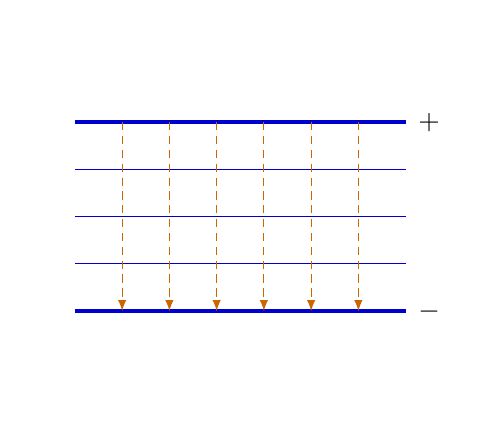
\begin{tikzpicture}[>=latex,scale=0.6]
  \useasboundingbox(-1,-2)rectangle(8,6);
  \foreach \x in {1,2,3}
  {
    \draw [blue!80!black](0,\x)--(7,\x);
  }
  \foreach \x in {0,4}
  {
    \draw[ultra thick,blue!80!black] (0,\x)--(7,\x);
  }
  \node at (7.5,0){$-$};
  \node at (7.5,4){$+$};
  
  \foreach \y in {1,2,...,6}
  {
    \draw[->,densely dashed,orange!80!black] (\y, 4)--(\y,0);
  }
\end{tikzpicture}
\end{document}